\documentclass{article}
\usepackage{graphicx}

\begin{document}

\title{CSE 6220 PA 1}
\author{Karl Hiner, Harshit Srivastava, Dalton Yu}
\date{}
\maketitle

Below is a chart showing the run-time of the program (in seconds) vs. the number of processors for $p = [1,2,..., 24]$.
This experiment was performed on the COC-ICE cluster.

\begin{figure}[htb]
    \centering 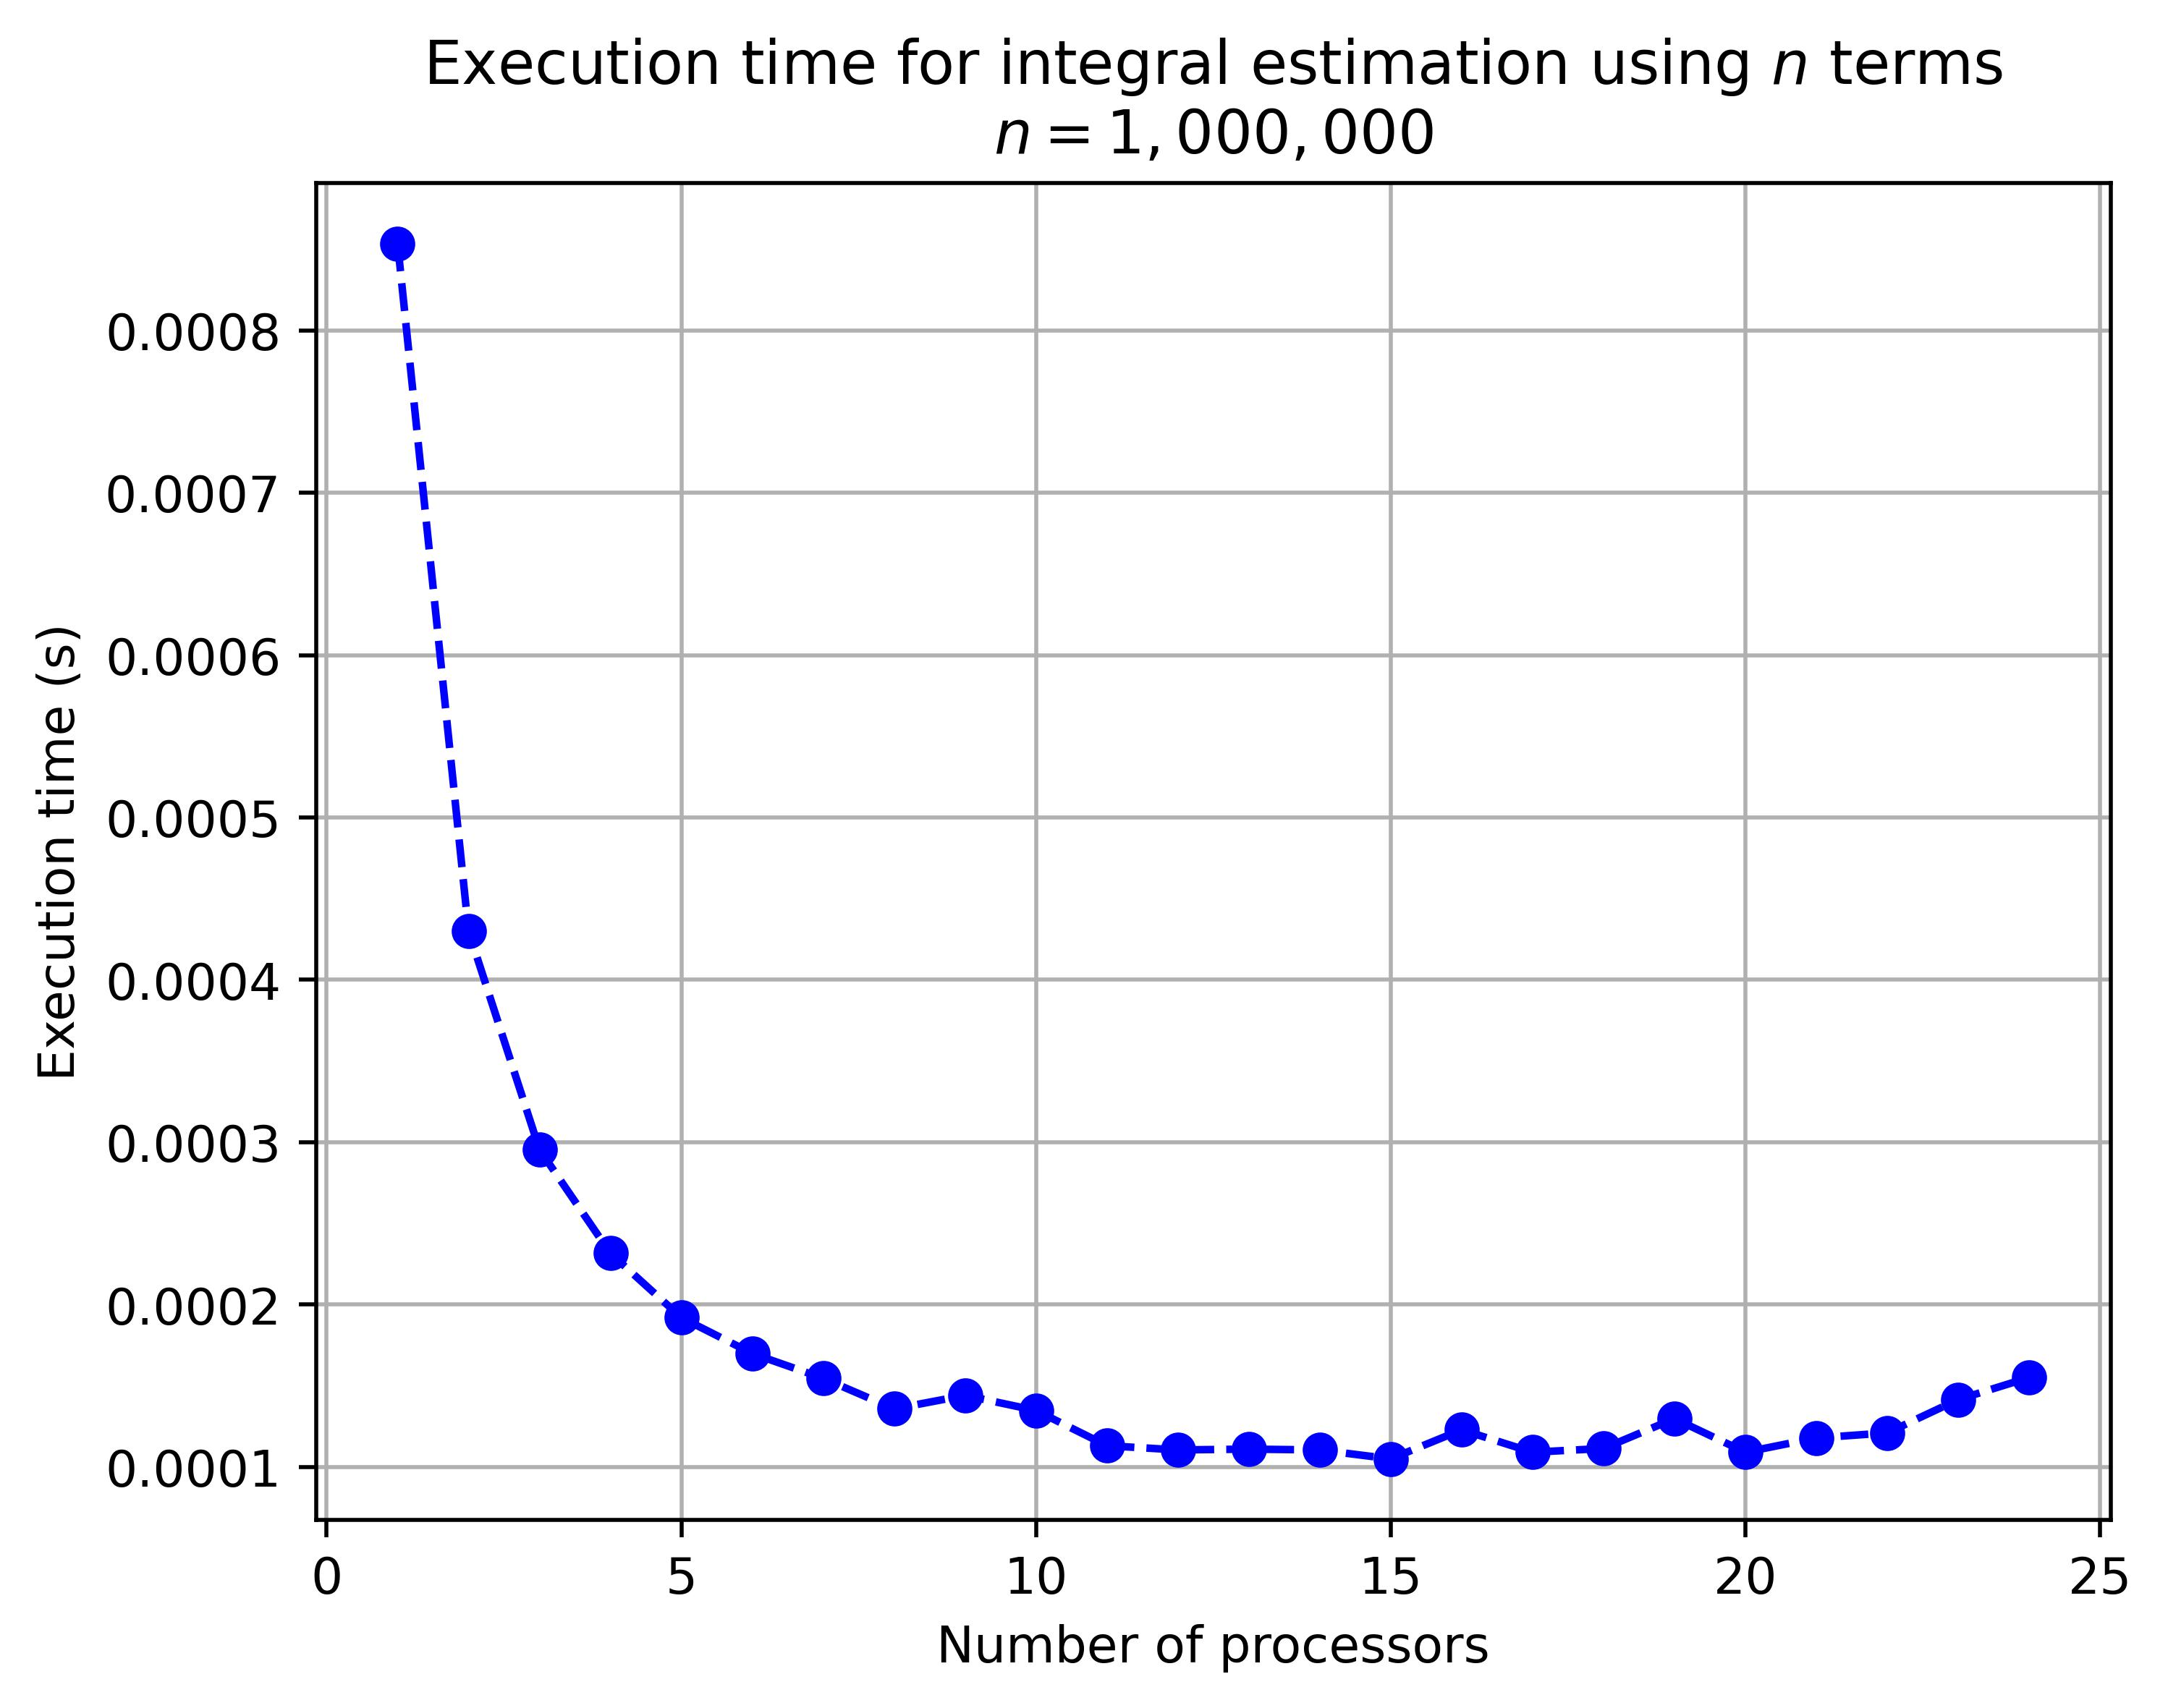
\includegraphics[width=\textwidth]{report_chart_n_1M_PACE.jpg}
    \caption{$n=10^6$, $p=[1,2,...,24]$ on PACE cluster}
    \label{fig:figure1}
\end{figure}

Note that this chart evaluates every value of $p$ in the tested range.
The execution time for $p = 2$ is very nearly half that of $p = 1$, showing a near-ideal speedup.
Likewise, $p = 4$ shows roughly a 2X speedup over $p = 2$, as expected for this embarrisingly parallel algorithm.

However, these speedups gradually decrease, reaching a minimum somewhere in the range $p \in [14, 20]$, and execution times even begin to consistently climb back up as $p > 20$.
This is because the communication overhead (such as latency and bandwidth) starts to overwhelm the speedup gained from parallel computation.

Note that with a problem size of $n=10^6$, using $p=20$ processors results in each process being responsible for $\frac{10^6}{20} = 5\cdot 10^4$ summation terms.
Calculating each term involves three multiplications and two additions for a total of five operations each.
Thus, we see communication overhead dominating the runtime when each processor is responsible for roughly $\leq \frac{1}{4}$M floating point operations.

\hbox{}

Note that we cap our processor count at $p=24$ since this experiment was run on the COC-ICE cluster, which has 24 cores per node.
Thus, after crossing $p=24$, we encounter dramatically higher execution times, due to inter-\textit{node} communication, which is much more costly than inter-\textit{core} communication.

This is clear from the following chart, which shows $p=[1,2,...,48]$:

\begin{figure}[htb]
    \centering 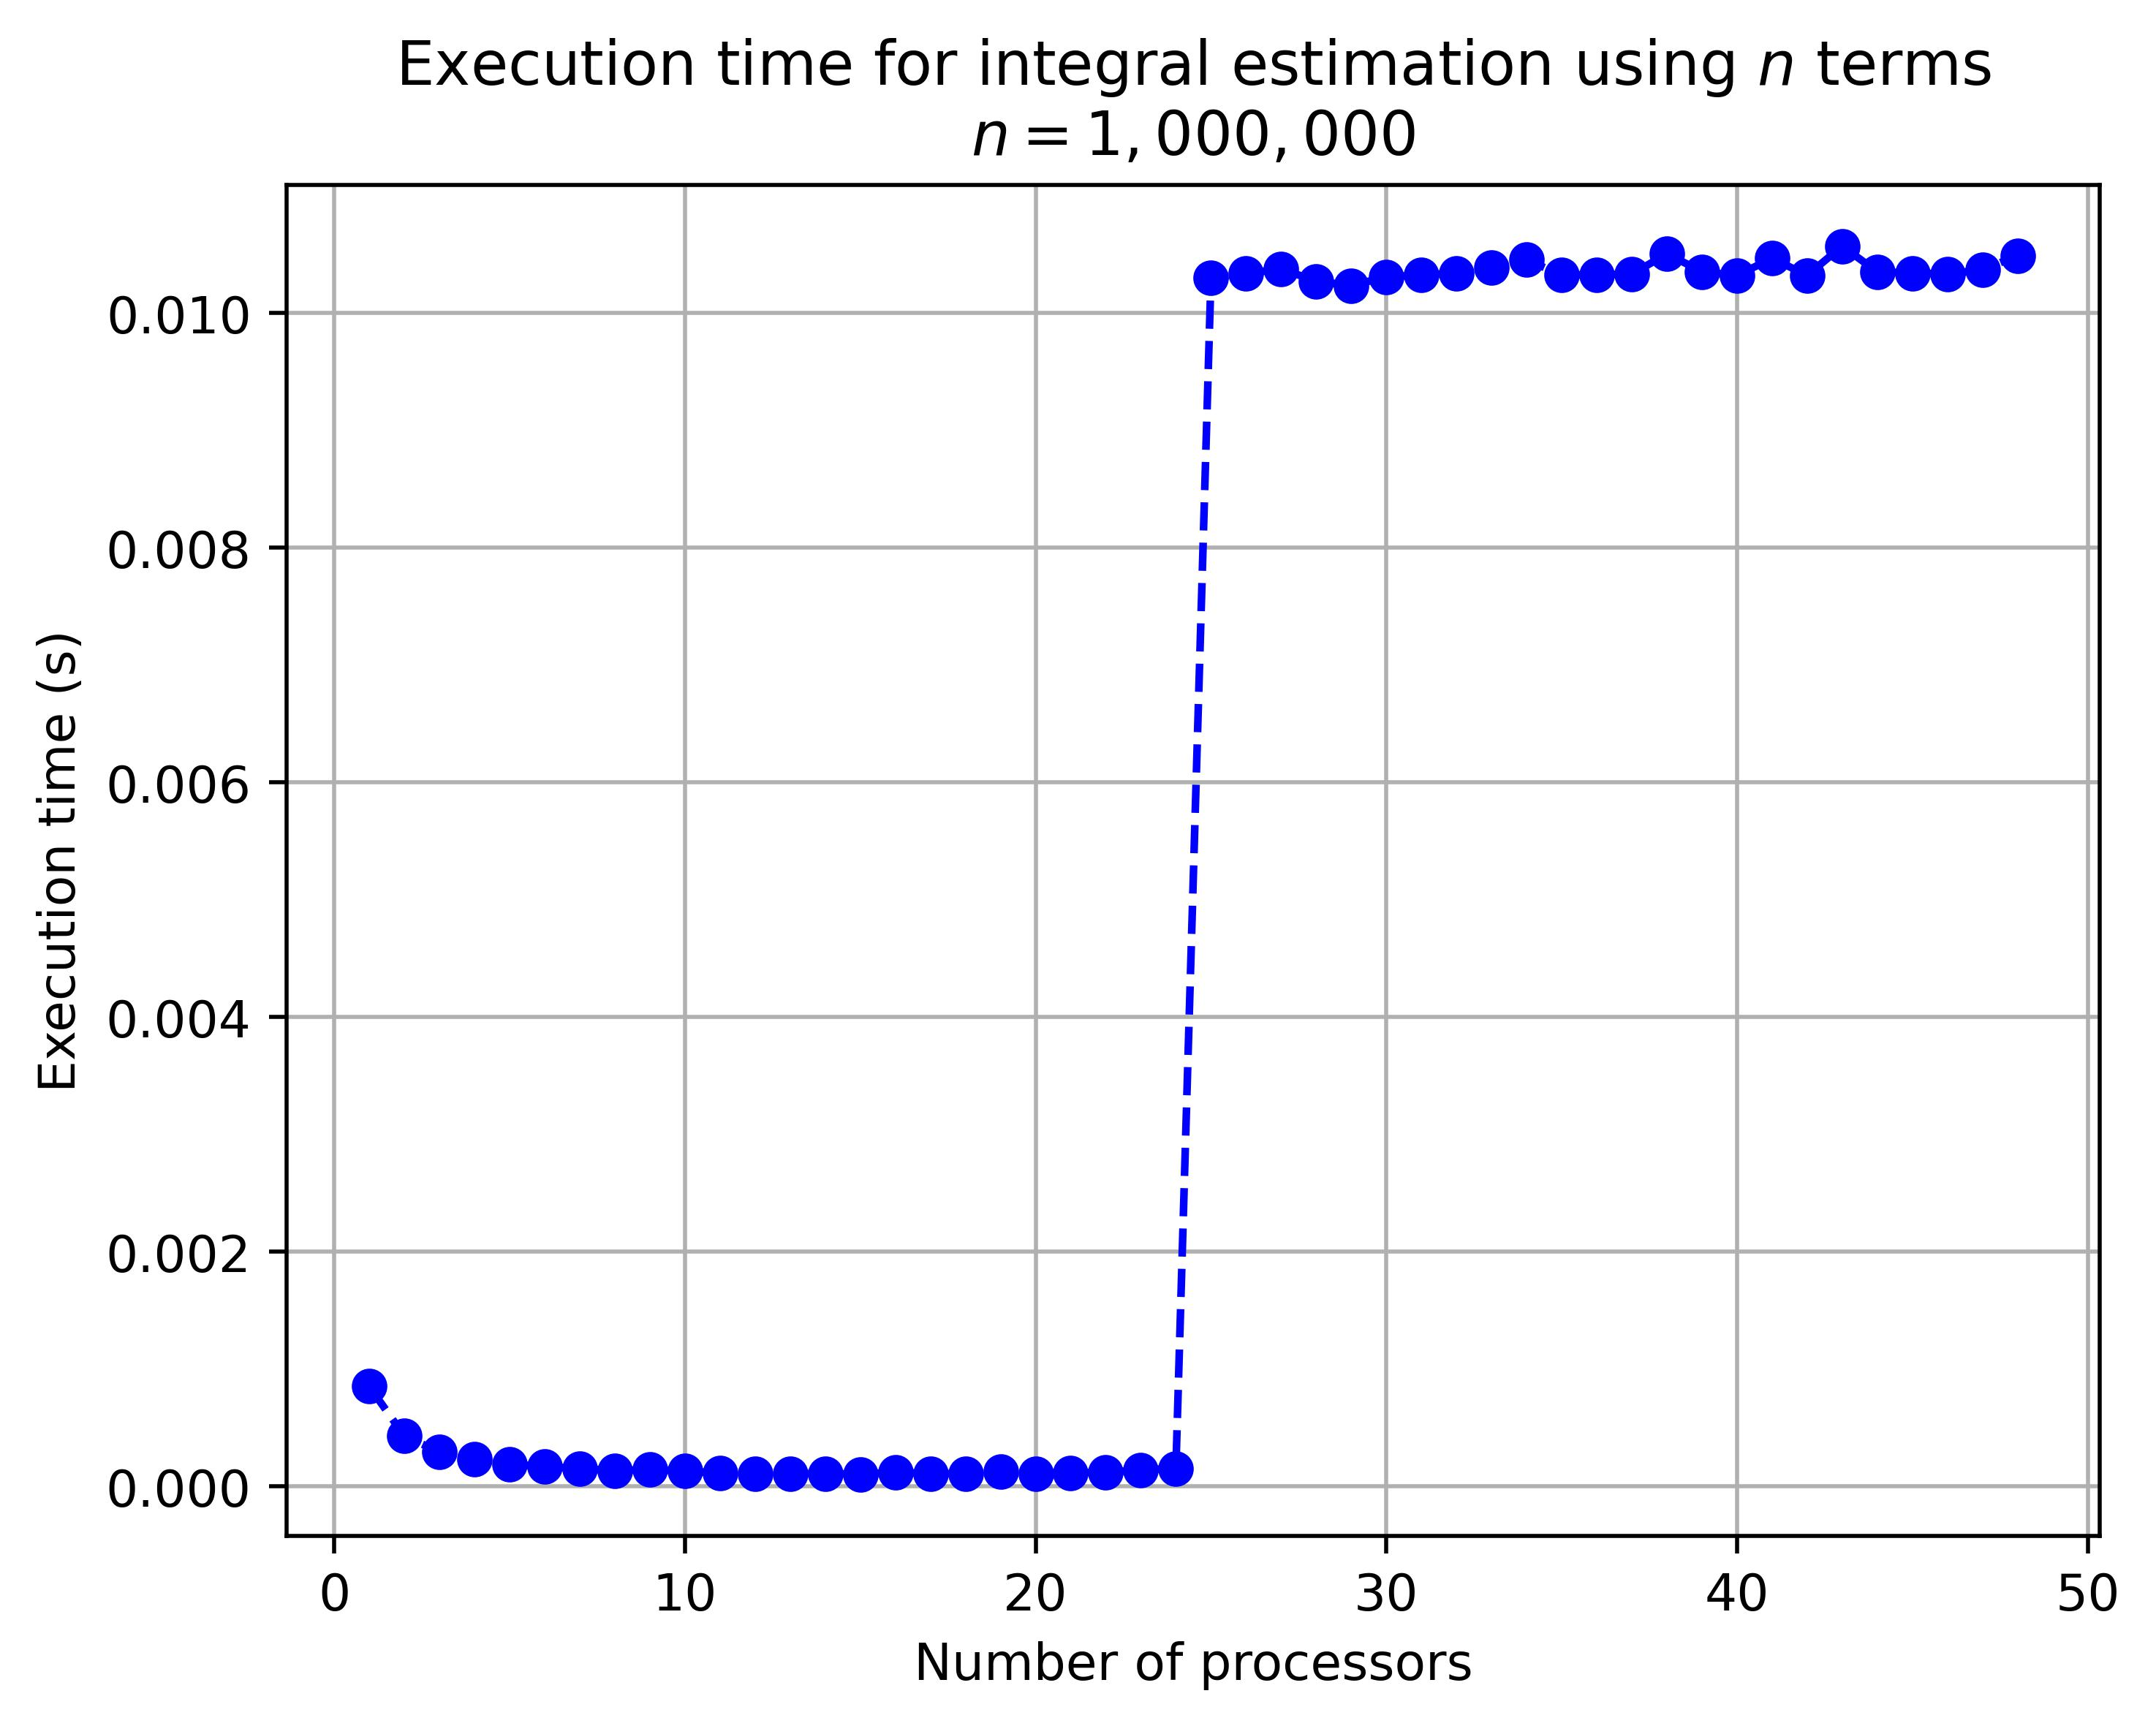
\includegraphics[width=\textwidth]{report_chart_n_1M_p_48_PACE.jpg}
    \caption{$n=10^6$, $p=[1,2,...,48]$ on PACE cluster}
    \label{fig:figure2}
\end{figure}

\end{document}
